\chapter{Informationserarbeitung}
\label{chap:Informationsbeschaffung}
Dieses Kapitel bietet fundamentale physikalische Gegebenheiten, sowie die relevanten Eigenheiten des verwendeten \ac{PIR}-Sensors. Da es sich um eine bildgebendes Messprinzip handelt, werden des Weiteren geometrische Aspekte erläutert. Schlussendlich bietet dieses Kapitel auch nötige Informationen über das Messobjekt bzw. die Messumgebung geliefert.

\section{Grid-Eye AMG8834}

Der verwendete Panasonic Grid-EYE AMG8834 ist ein bildgebender \ac{MEMS}-Sensor, der mit insgesamt 64 temperaturempfindlichen Thermosäulenelementen ausgestattet ist. Alle nachfolgenden Angaben sind, wenn nicht anders angegeben aus den Datenblätter zu entnehmen.

\begin{figure}[H]
	\centering
	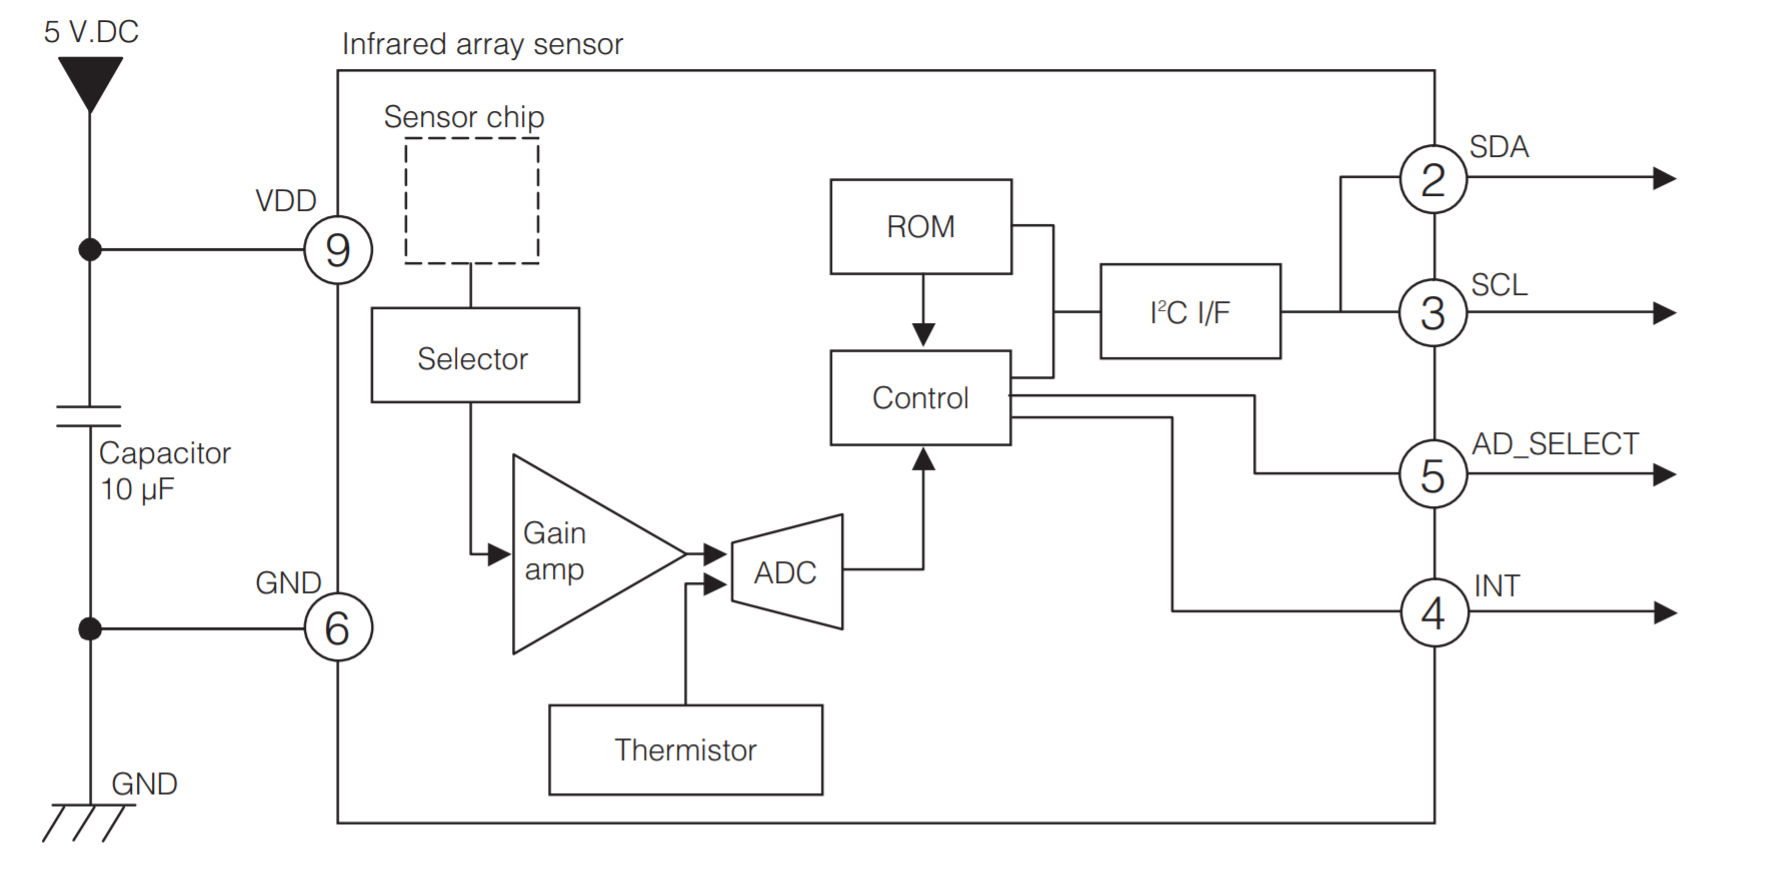
\includegraphics[width=0.75\textwidth]
	{fig/Circuit_AMG8834.PNG}
	\caption[Schema des AMG8834 Sensors]{Schema des AMG8834 Sensors} \protect\cite{AMG8834}
	\label{fig:SchemaAMG8834}
\end{figure}


In Abbildung \ref{fig:SchemaAMG8834} ist das Prinzipschema des Sensors darstellt. Das Messprinzip des Sensors wird im Unterkapitel \ref{seebeck} detailliert erläutert. Die entstandene Spannung wird durch die \ac{ASIC} des \ac{MEMS}-Sensor verarbeitet. Das selektierte Thermoelement wird verstärkt, mit dem integrierten Thermistor verglichen und mit dem \ac{ADC} gewandelt. Über die \ac{I2C}-Schnittstelle lassen sich die Werte der Thermoelemente und der Thermistoren je aus 2 Register auslesen. Die Messwerte werden alle 100 ms aktualisiert. 
 
Dabei werden lediglich 12 Bit für die Pixelwerte genutzt, welches zur kleinsten unterscheidbaren Größe von 0.25 $^\circ$C führt. Die Thermistor-Register lassen sich mit der Auflösung von 0.625 $^\circ$C unterscheiden. Dies

Durch die hohe interne Verstärkung besitzt der Sensor jedoch bei normalen Bedingungen\footnote[2]{Umgebungstemperatur 0-80 $^\circ$C bei Luftfeuchtigkeit 15-85\%} lt. Datenblattangaben eine Genauigkeit von +/- 3°C. 





Der Sensor AMG8834 ist standardmäßig auf einen Emissionsgrad von $\epsilon$ =0.93 kalibriert.

\begin{figure}[H]
	\centering
	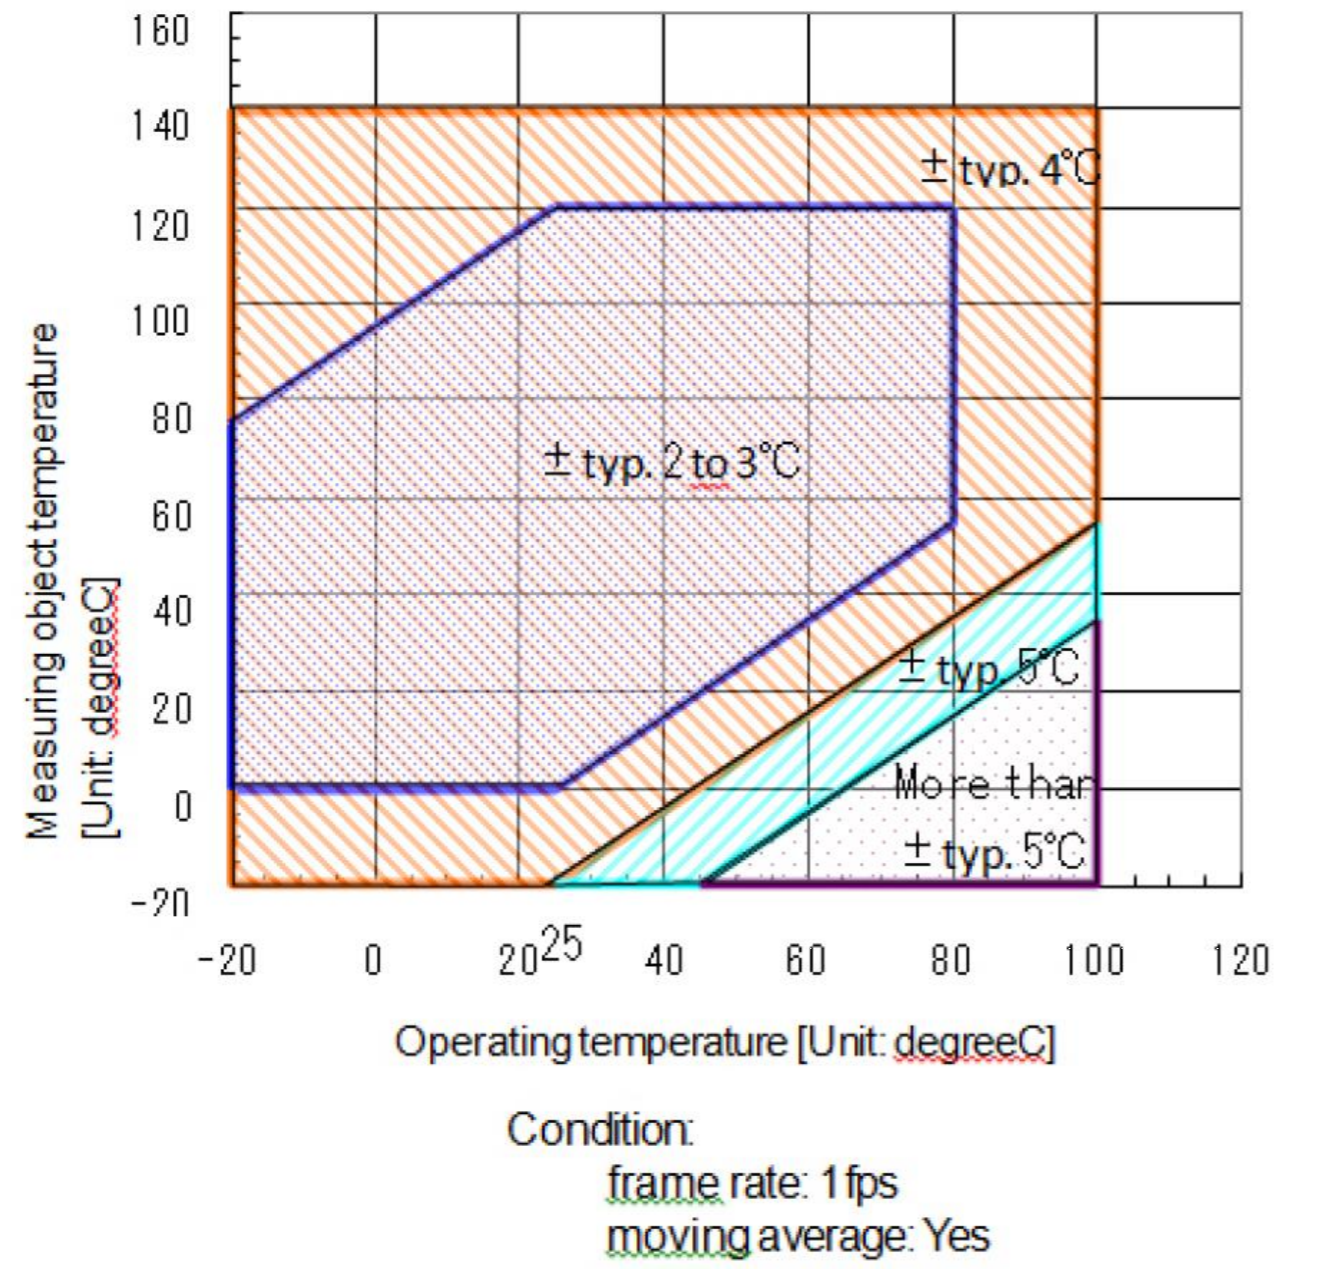
\includegraphics[width=0.6\textwidth]
	{fig/accuracy.PNG}
	\caption[Messgenauigkeit]{Messgenauigkeit} \protect\cite{AMG8834}
	\label{fig:Temperaturbereich}
\end{figure}


Die eintreffenden Infrarotwellen werden durch die Silizium Linse gefiltert. Dabei treten lediglich langwellige  Infrarotstrahlungen mit den Wellenlängen 8-13 $\mu$m durch die Linse. Dies entspricht dem dritten atmosphärischen Fenster.


\ac{ASIC}

\begin{figure}[H]
	\centering
	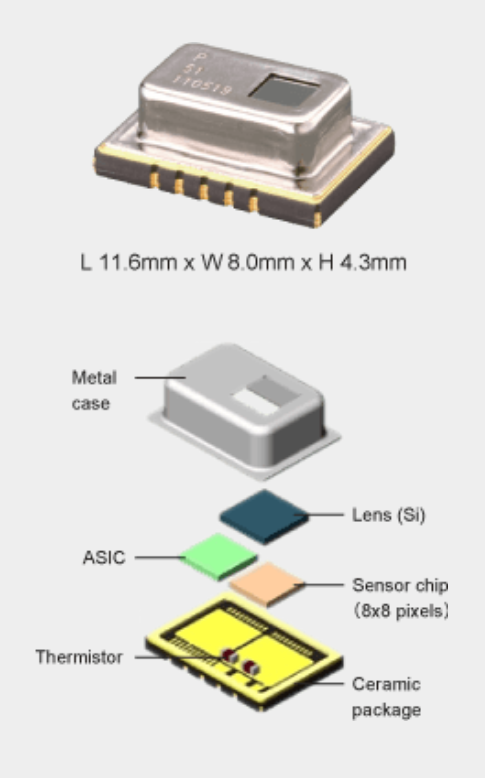
\includegraphics[width=0.3\textwidth]
	{fig/grid_eye_aufbau.PNG}
	\caption[Schema des AMG8834 Sensors]{Schema des AMG8834 Sensors} \protect\cite{AMG8834}
	\label{fig:Explosionsdarstellung}
\end{figure}







\begin{figure}[H]
	\centering
	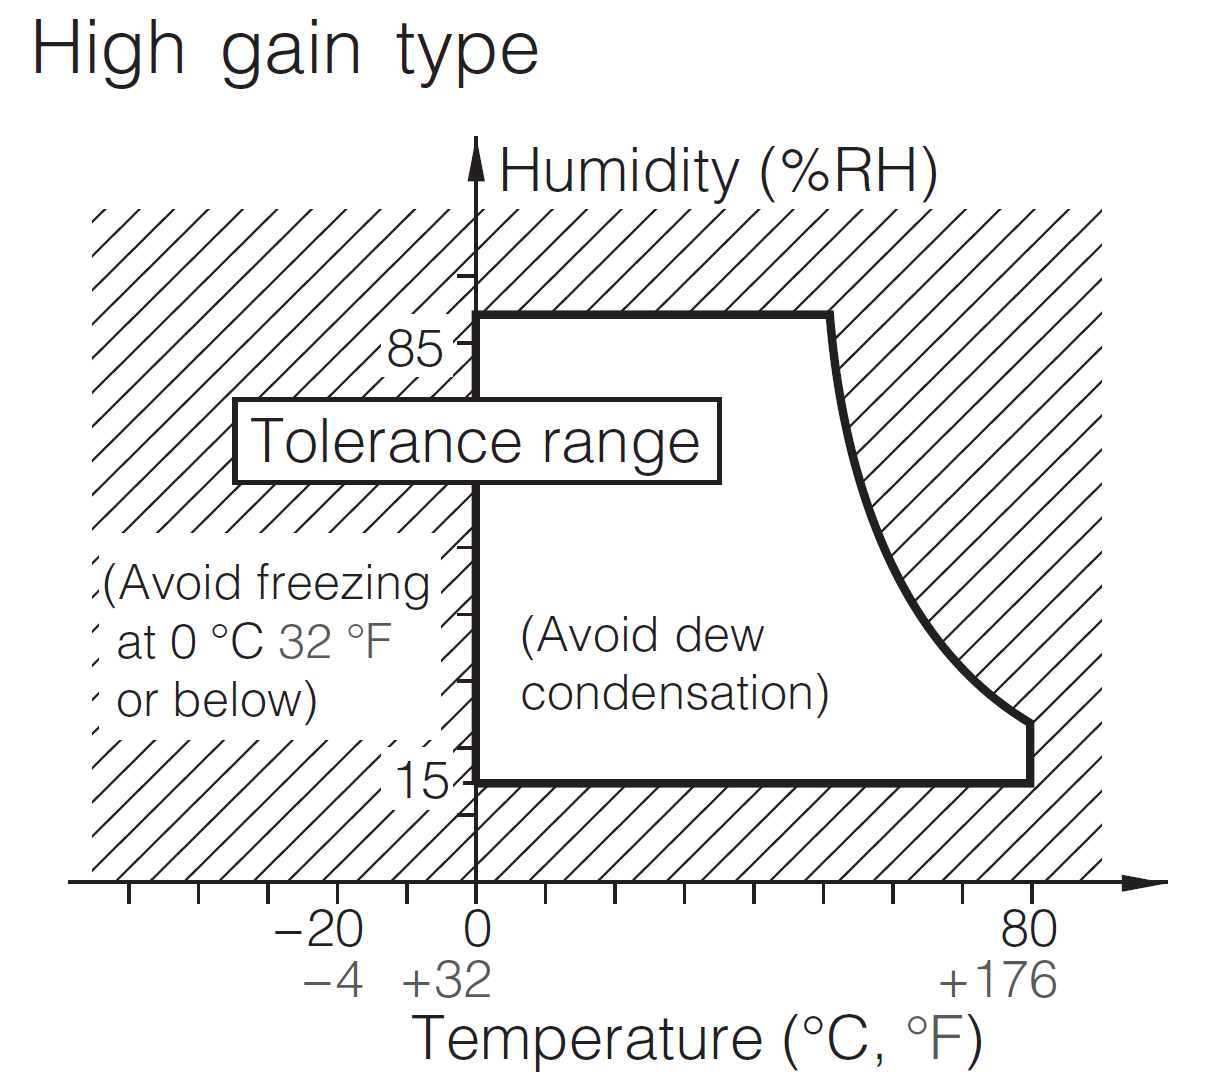
\includegraphics[width=0.5\textwidth]
	{fig/Humidity_Tolerance.PNG}
	\caption[Einfluss Luftfeuchtigkeit]{Einfluss Luftfeuchtigkeit} \protect\cite{AMG8834}
	\label{fig:Humidity}
\end{figure}


\section{Physikalische Aspekte}

Dieser Abschnitt erläutert auf kurze und prägnante Weise, physikalischen Aspekte dem Sensor zu Grunde liegen. Dies bietet die Grundlage für die Bestimmung der Störquellen und das Verhalten des Sensors bei entstprechenden äusseren Einwirkungen. 



\begin{table}[H]
	\begin{tabular}{l|c|c}
		
		\rowcolor{gray} Grösse &  Bezeichnung  & Einheit \\
		\hline 
		Wärmestrom &  $\dot{Q}$ & $J$  \\ 
		\rowcolor{gray}Emission & $\epsilon$ & $-$\\	
		Reflektion &  $\rho $ & $-$ \\
		\rowcolor{gray} Transmission & $\tau$ & $-$\\
		Absoprtion &  $\alpha$ & $-$  \\ 
		
		\rowcolor{gray}Geschwindigkeit des Chassis & $\dot{Q}$ & $m/s$\\
		spektrale spezifische Ausstrahlung &  $M_{\lambda }$ & $m/s^2$ \\
		\rowcolor{gray} Planksches Wirkungsquantum &  $ h$ & Js \\ 
		Lichtgeschwindigkeit im Vakuum & $c $ & $ m/s$ \\ 
		\rowcolor{gray} Stefan-Boltzmann-Konstante & $\sigma$ & $ rad/s^2 $ \\ 
	\end{tabular}
	\caption{Legende physikalische Grössen Konzeptzeichnungen}
	\label{tab:Legende Physikalische Grössen} 
\end{table} 


\subsection{Allgemein}



\begin{table}[]
	\centering
	\label{my-label}
	\begin{tabular}{|l|l|l|}
		\hline
		\rowcolor{gray} IR-A {[}$\mu$m{]} & IR-B {[}$\mu$m{]} & IR-C {[}$\mu$m{]} \\ \hline
		0.78 - 1.4  & 1.4 - 3.0   & 3 - 1000    \\ \hline
	\end{tabular}
	\caption{Infrarotbereiche}
\end{table}


Formel für die spektrale spezifische Ausstrahlung  eines Schwarzkörpers der absoluten Temperatur  T. Für sie gilt

\begin{equation}
\label{eq5}
M_{\lambda } = \frac{2\pi h c^2 }{\lambda^5}*\frac{1}{e^\frac{hc}{\lambda k_{B}}-1}
\end{equation}
\myequations{Plank'sches Strahlungsgesetz}

Das Stefan-Boltzmann-Gesetz gibt die Strahlungsintensität Q eines idealen Temperaturstrahlers an (Integral des Plank'schen Gesetzes über alle Wellenlängen). Diese Intensität ist proportional zur 4. Potenz der absoluten Temperatur. Es lautet:
Strahlungsleistung

\begin{equation}
\label{eq1}
\frac{\mathrm{d} Q}{\mathrm{d} t} = \epsilon *\sigma * A * T^4
\end{equation}
\myequations{Wärmestrahlung}






Ein grauer Körper im Sinne der Strahlungsphysik ist ein Körper, dessen Oberfläche auftreffende Strahlung nicht vollständig absorbiert und dementsprechend auch nicht bei einer gegebenen Temperatur die maximale Strahlung (Schwarzkörperstrahlung) emittiert (siehe plancksches Strahlungsgesetz). Er hat jedoch einen wellenlängenunabhängigen Emissions- bzw. Absorptionsgrad - er erscheint „grau“, wobei sich die fehlende „Farbe“ nicht auf den sichtbaren, sondern auf den für die Messung relevanten Bereich des Spektrums bezieht.

\begin{equation}
\label{eq2}
a^2+b^2=c^2
\end{equation}
\myequations{Planksches Strahlungsgesetz}


\begin{equation}
\label{eq4}
\epsilon = \alpha  = 1
\end{equation}
\myequations{Strahlung Energieerhaltung Festkörper}

\begin{equation}
\label{eq4}
\epsilon = \varphi  = 1
\end{equation}
\myequations{Schwarzer Stahler, Energieerhaltung}



\subsection{Seebeck-Effekt}
\label{seebeck}

Die durch die konvexe Linse gesammelten infrarotstrahlen verursachen auf den einzelnen Thermosäulenelemente, dass die Oberfläche erwärmt wird. 


\begin{figure}[H]
	\centering
	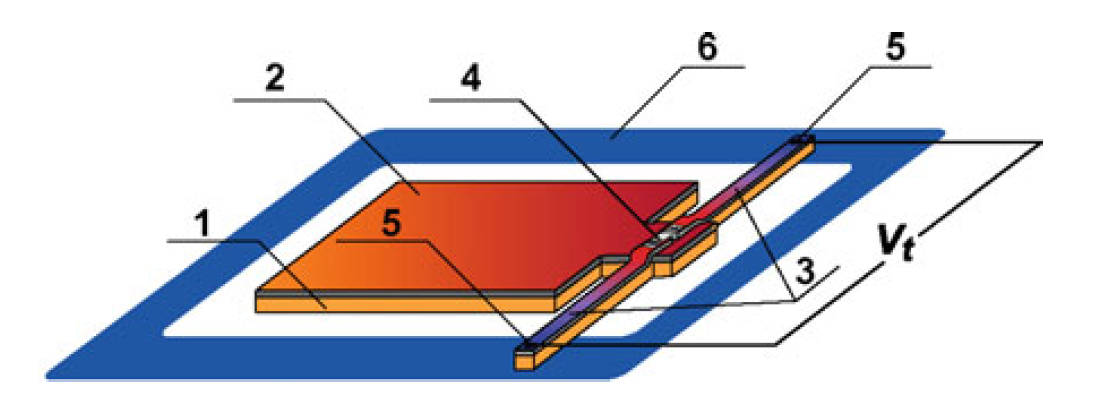
\includegraphics[width=0.5\textwidth]
	{fig/Mems_Thermopile.PNG}
	\caption[Aufbau Thermosäule]{Aufbau Thermosäule} \protect\cite{AMG8834}
	\label{fig:AufbauThermo}
\end{figure}

\begin{equation}
\label{eq4}
\alpha + \varphi + \tau  = 1
\end{equation}
\myequations{Schwarzer Stahler, Energieerhaltung}



\section{geometrische Aspekte}

Im vorherigen Abschnitt wurden bereits erwähnt, dass durch den begrenzten \ac{FOV} des Sensors die Distanz zum Messobjekt eine entscheidende Rolle spielt. In der nachstehenden Skizze (Abbildung \ref{}) sind die Verhältnisse perspektivisch dargestellt. Dabei wird von einer Raumhöhe von 2.10 m ausgegangen. (nach Standardkabine EN 81-70)   

\begin{figure}[H]
	\centering
	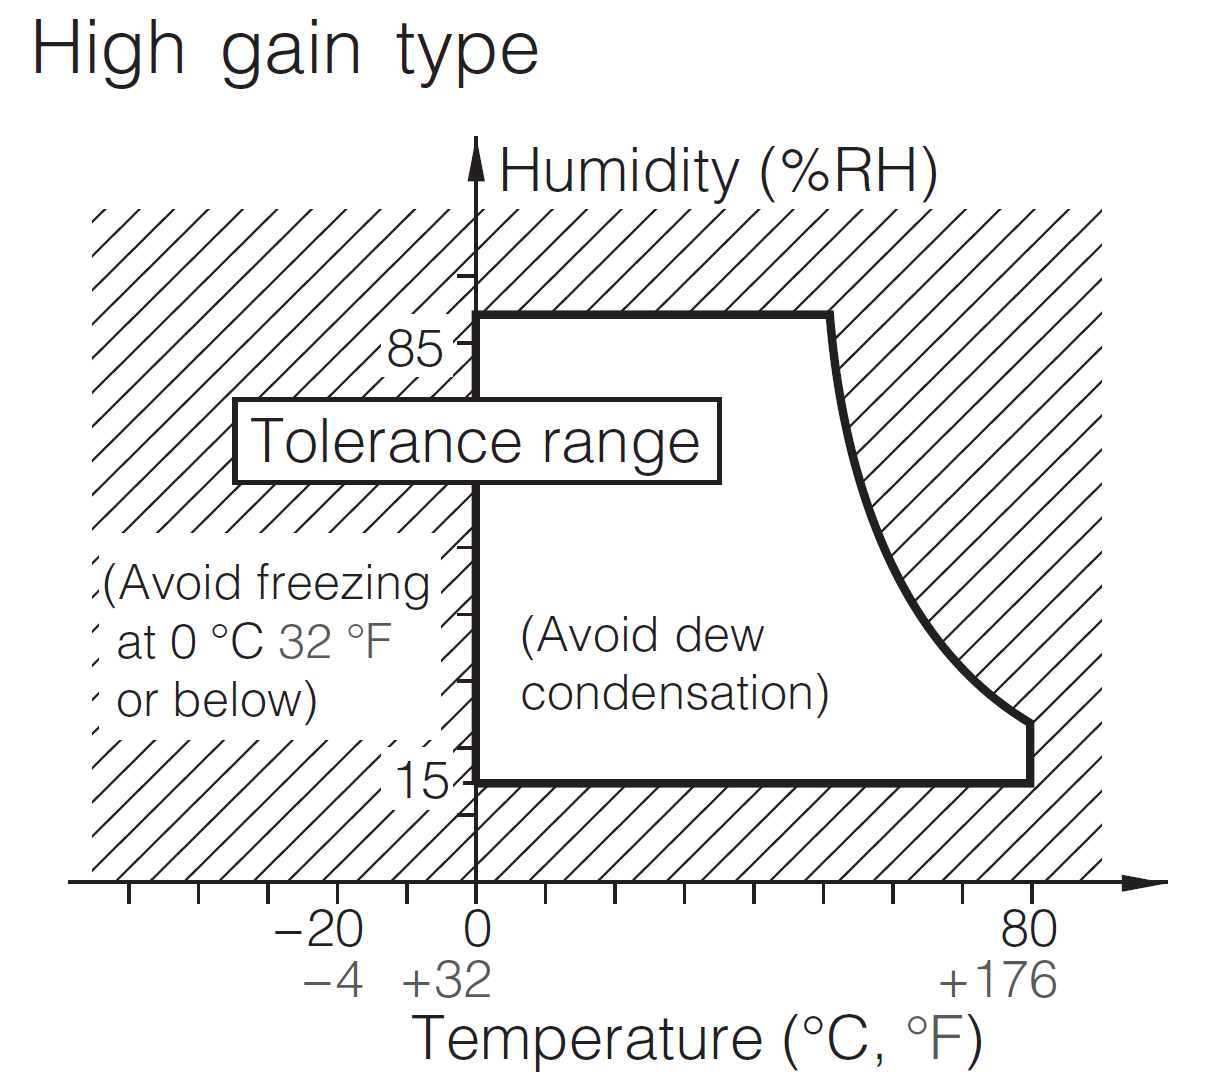
\includegraphics[width=0.5\textwidth]
	{fig/Humidity_Tolerance.PNG}
	\caption[Einfluss Luftfeuchtigkeit]{Einfluss Luftfeuchtigkeit} \protect\cite{AMG8834}
	\label{fig:Geometrie}
\end{figure}

Die räumliche Streckungen verursacht zusätzlich eine perspektivische Verzerrung, welcher in dieser Betrachtung nicht weiter beachtet wird. Zu sehen ist jedoch deutlich, dass bei der Messung von Personen die Messdistanz zwischen 10 bis 110 Zentimeter am relevantesten ist. In diesem Bereich kann jedoch mit dem aktuellen \ac{FOV} im besten Fall eine Fläche von 0.666 $ m/s^2 $ abgedeckt werden. Um eine Aufzugkabine mit 8 Personen\footnote[1]{Masse: (HxBxT) 2100 x 1100 x 400 [mm]} mit entsprechenden Messdistanzen wird ein Öffnungswinkel von -XX$^\circ$ benötigt. 
)

Problematisch kann in diesem Zusammenhang die Abschattung des Messbereichs durch grosse Personen sein, welche zentral positioniert sind. 

 

\section{Messobjekt und Messumgebung}

Dieses Kapitel beschreibt die Erkenntnisse bei der Betrachtung des Messobjekts und der Messumgebung. Dabei wurden einerseits die Kennwerte von Personen zusammengetragen, sowie die Messumgebung auf Störquellen und Einflussfaktoren begutachtet. Dank der Firma ARLEWO AG konnten unterschiedliche Aufzüge vermessen und bewertet werden. 

\subsection{Personen}



Die Reaktionen im menschlichen Körper sind auf eine Kerntemperatur von 37 °C eingestellt mit einer Toleranz von etwa + 0,5 Kelvin (Grad). Am kältesten ist die Haut, die etwa 4 bis 7 Kelvin (Grad) kälter ist. Die Aufteilung der verschiedenen Arten der Wärmeabgabe beträgt bei einem ruhenden Menschen in einer Umgebung von 20 °C:

\begin{enumerate}
\item 
\begin{itemize}
	\item  46 \% Strahlung
	\item  33 \% Konvektion
	\item  19 \% Schwitzen
	\item   2 \% Atmung.
\end{itemize}
\end{enumerate}	


Die Höhe der biologisch notwendigen Wärmeabgabe hängt im wesentlichen
- von der Schwere der Tätigkeit und
- von der Größe der Körperfläche 
und damit von der Körpergröße des Menschen ab.

Bei einer Veränderung der oben genannten Voraussetzungen verschieben sich die Anteile. Herrscht ein starker Wind, so erhöht sich der Anteil der Konvektion.

Diese Art der Wärmeabgabe nimmt mit der Umgebungstemperatur bis zum Wert null bei 36 °C ab. Hat die Umgebung nämlich die Körpertemperatur erreicht, kann folglich durch Strahlung und Konvektion keine Wärme mehr abgeführt werden.

Der schraffierte Bereich gibt die Höhe dieser Art der
Wärmeabgabe an. In einer Umgebung mit Temperaturen oberhalb 37 °C kann also die Wärme
nur noch durch Schwitzen abgeführt werden. Bei mittelschwerer Arbeit verdoppelt sich
ungefähr die Wärmeabgabe des Menschen gegenüber dem ruhigen Sitzen, da die Muskeln,
wie bereits erwähnt, zu 80 \% Abwärme erzeugen. Bei schwerer Arbeit kann die Wärmeabgabe auf ca. 300 W ansteigen. Trainierte Sportler können noch höhere Leistungen erzeugen.

\begin{figure}[H]
	\centering
	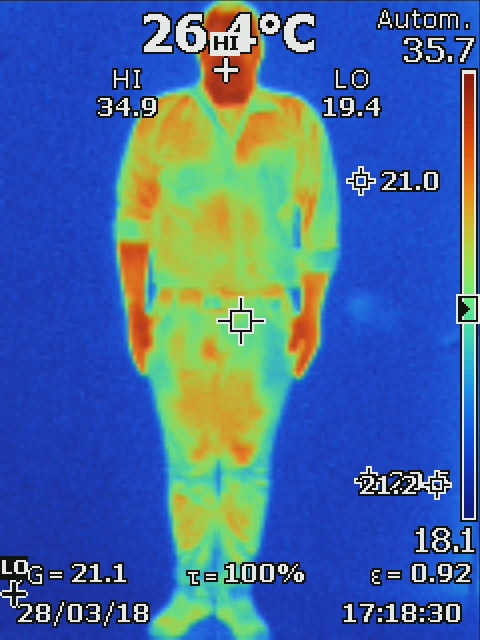
\includegraphics[width=0.3\textwidth]
	{fig/person_waerme.JPG}
	\caption[Wäermebild eines Probanden]{Wärmebild eines Probanden}
	\label{fig:Waermebild}
\end{figure}


Die
Wärmeabgabe des Menschen ist also proportional seiner Oberfläche und damit von der Körpergröße abhängig. Die Oberfläche eines normalen Menschen beträgt ungefähr 2 m2.

Ein nackter Mensch hat beispielsweise einen k-Wert von
ungefähr 10 W/(m2·K). Damit ergibt sich aus der obigen Gleichung der Wärmestrom von 120
W für eine Umgebungstemperatur von 26 °C. \cite{MenschWaerme}

\subsection{Personenaufzüge}

In diesem Unterkapitel wurde das Messobjekt "Personenaufzug" näher betrachtet. Neben räumlichen Parametern wie Höhe, Grundfläche und Volumen spielen vor allem die Oberflächenbeschaffenheit bzw. das Oberflächenmaterial eine wichtige Rolle. Weitere thermische Einflussfaktoren finden sich in der Umgebungstemperatur und der eingebauten Leuchtmittel.



In Abbildung \ref{fig:Edelstahlgewalzt} und \ref{fig:Edelstahlmatt} sind 
\begin{figure}[H]
	\centering
	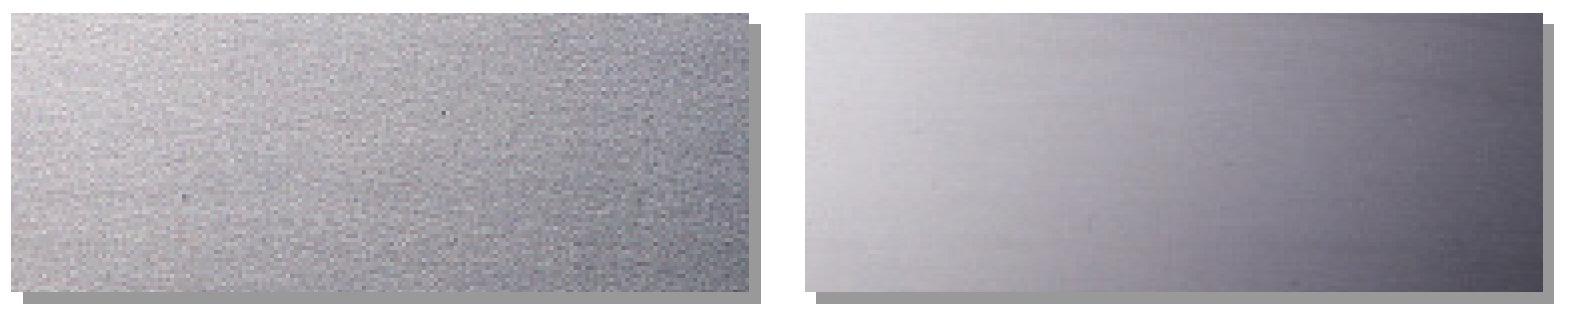
\includegraphics[width=0.8\textwidth]
	{fig/Edelstahl_gewalzt.PNG}
	\caption[Schema des AMG8834 Sensors]{Schema des AMG8834 Sensors} \protect\cite{Edelstahl}
	\label{fig:Edelstahlgewalzt}
\end{figure}


\begin{figure}[H]
	\centering
	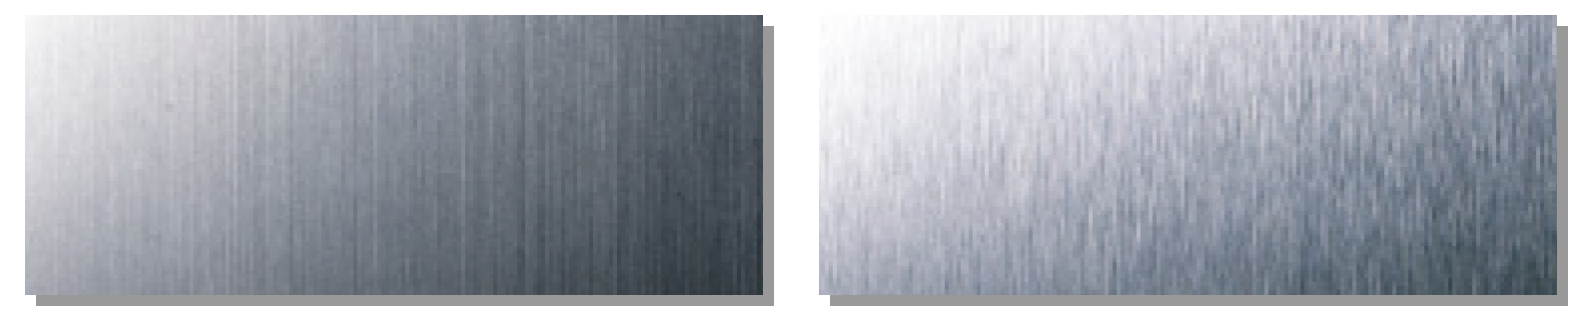
\includegraphics[width=0.8\textwidth]
	{fig/Edelstahl_matt.PNG}
	\caption[Schema des AMG8834 Sensors]{Schema des AMG8834 Sensors} \protect\cite{Edelstahl}
	\label{fig:Edelstahlmatt}
	
	
\end{figure}

\section{Störquellen}

Einflüss Luftströme





\section{verwendete Software}



\section{Fazit}

